%% Compilation Notes:
%   Turns out, 100 samples per 2D graph and a 3D graph with 100 samples is expensive, so this takes a while...
%   Spam enter on all the 'errors'
%   Might need to immediately recompile it after compiling it the first time to get rid of extra page and to 
%       ensure equation/figure references are processed correctly


\documentclass[nofoot,pdf-a,balance,colorlinks,upint,subscriptcorrection,varvw,mathalfa=cal=boondoxo]{asmeconf}
\special{papersize=8.5in,11in}

\usepackage{amsmath}
\usepackage{mathtools}
\usepackage{amssymb}
\usepackage{xfrac}
% \usepackage[margin=1.00in]{geometry}
% \usepackage{tabto}
\usepackage{tikz}
\usepackage{pgfplots}
\usepackage[thinc]{esdiff}
\usepackage{float}

\pgfplotsset{
    compat = newest,
    /pgf/declare function= {
        % y(t)
        f(\x) = 160.3981*(\x)^4-105.7772*(\x)^3+14.7141*(\x)^2+0.4;
        % derivative of y(t)
        g(\x) = 160.3981*4*(\x)^3-105.7772*3*(\x)^2+14.7141*2*(\x);
        % second derivative of y(t)
        h(\x) = 160.3981*12*(\x)^2-105.7772*6*(\x)+14.7141*2;
    },
}

% for the autumn color library
\usepgfplotslibrary{colormaps}


% added for compliance because LaTeX was warning me that I'm supposed to have a pdftitle defined
\hypersetup{
	pdfauthor={Lucas S. Johnston, Brendan Moskalik},
    pdftitle={Solution for the Dynamics Robot Arm Project},
	pdfkeywords={Dynamics, Robot Arm Project},
	pdfsubject = {Solution for the Dynamics Robot Arm Project},
}

\begin{document}
    \ConfName{Proceedings of the Dynamics 2024\linebreak Very Local Mechanical Engineering Congress and Exposition}
    \ConfDate{Spring, 2024} % update 
    \ConfCity{Spokane, WA}

    \title{Robot Arm Project}
    \SetAuthors{Lucas S. Johnston\affil{1}\JointFirstAuthor, Brendan Moskalik\affil{1}\JointFirstAuthor}
	\SetAffiliation{1}{Gonzaga University, Spokane, WA}

    \maketitle

    \section*{Problem Description}
	
    Given an egg in free fall, we want to determine a smooth path over time that a robotic arm can follow to catch the egg without it breaking. The robotic arm consists of a linear actuator and a motor that rotates the linear actuator such that it's motion can be fully described by $r\left(t\right)$ and $\theta\left(t\right)$, which are the radius as a function of time and the angle as a function of time, respectively. In the name of good faith and best practice, all angles discussed will be in radians. Together with the physical constraints imposed on the system that lock the robotic arm's catcher onto a straight line, these both fully define a function $y\left(t\right)$, which describes the height of the catcher from when it starts until it reaches its final position. Helpfully, $y\left(t\right)$ fully describes both $r\left(t\right)$ and $\theta\left(t\right)$, so our primary goal, first and foremost, is to solve for a valid $y\left(t\right)$ function. The arm must start at rest 0.6 meters above the table surface. To smoothly catch the egg, the arm must match the position, velocity, and acceleration of the egg at some instance around 0.5 meters above the table. The egg starts at rest 0.8 meters above the table. The catch must be complete with the arm stopped moving at least 0.1 m above the table as well. \newline \newline 
    For our purposes, we will define the origin to be O, the pivot point of the robot arm. Let $f\left(t\right)$ be the function representing the free fall of the egg. Both $y$ and $f$ are defined as the height above this origin point, in meters. This means $y\left(t\right)$ must satisfy the following conditions:
    \begin{equation}\label{condition_1}
        y\left(0\right) = 0.4
    \end{equation}
    \begin{equation}\label{condition_2}
        \dot{y}\left(0\right) = 0
    \end{equation}
    \begin{equation}\label{condition_3}
        {y}\left(t_1\right) = f\left(t_1\right) 
    \end{equation}
    \begin{equation}\label{condition_4}
        \dot{y}\left(t_1\right) = \dot{f}\left(t_1\right)
    \end{equation}
    \begin{equation}\label{condition_5}
        \ddot{y}\left(t_1\right) = \ddot{f}\left(t_1\right)
    \end{equation}
    \begin{equation}\label{condition_6}
        {y}\left(t\right) > 0.1 \textrm{    } \forall t > 0
    \end{equation}
    \begin{equation}\label{condition_7}
        \exists \textrm{ }t > t_1 \textrm{      such that  }\dot{y}\left(t\right) = 0 
    \end{equation}
    Here $t_1$ is defined as the time when the robot arm catches the egg.
    \begin{equation}\label{condition_8}
        \exists\textrm{  } t_1 \textrm{      such that  } f(t_1) \approx 0.3
    \end{equation}
	
		\section*{Assumptions}
	
	\begin{itemize}
        \item We are on earth and that $g = 9.81 \textrm{ }\sfrac{\textrm{m}}{\textrm{s}^2}$
		\item There is negligible drag
		\item There is negligible flex in the robot arm
        \item We have enough precision in our control of the motors to implement any arbitrary, smooth function that won't crash the arm
		\item The robot knows when the egg drops, and can start motion at that exact time
	\end{itemize}

	\section*{Solution Methods}
	
		Our solution methods were to first find the position, velocity and acceleration of the egg at the point where we wanted to start the catch. We then used this data as well as the initial conditions of the arm to find a function where the arm would match these data points. We had 5 data points, so we constructed it as a constant snap function (which gave us 5 unknowns to solve for). We then used this resulting function and parameterized it to find $r\left(t\right)$ and $\theta\left(t\right)$. These are the position functions of our actuators of the robotics arm and describe the motion of it.\newline

        To begin, we want to find a function $f\left(t\right)$ that describes the egg in free fall. This gives us the following:

        \begin{equation}
            f\left(t\right) = 0.6 - \frac{1}{2} \cdot 9.81 t^2
        \end{equation}
        \begin{equation}
            \dot{f}\left(t\right) = - 9.81 t
        \end{equation}
        \begin{equation}
            \ddot{f}\left(t\right) = - 9.81
        \end{equation}

         So far, our problem is a little `under-constrained,' so let's explicitly define $t_1$.
         \begin{equation} 
             f(t_1) = 0.3 \implies t_1 = \sqrt{\frac{0.6}{9.81}} \approx 0.24731
         \end{equation}
     
       Initially, we tried a number of methods to find a function for $y$. We tried assuming a constant jerk, and integrating backwards, using initial conditions to solve variables. 
    \begin{equation*}
        \dddot{y} = A
    \end{equation*}
        We tried using an offset sine wave, since it'll oscillate to a constant velocity and can smoothly change all of its time derivatives of position.
    \begin{equation*}
        y = A \cdot \sin{\left(\omega t + \phi\right)} + B
    \end{equation*}
        When that didn't work out, we tried damped sine waves as well.
    \begin{equation*}
        y = A \cdot \sin{\left(\omega t + \phi\right)}\cdot e^{-st} + B
    \end{equation*}

    In the end, we realized that, if you look at Eq. \eqref{condition_1} through \eqref{condition_5}, you'll see we essentially have five defined points our function has to go through (if you broaden points to include a fixed position at a certain time, a fixed velocity at a certain time, or a fixed acceleration at a certain time). In the wise words of Brook Taylor, ``Everything [smooth] is a polynomial if you have enough terms.''\footnote{He did not actually say this.} Furthermore, in a rare instance of physicists being practical, Richard Feynman said ``I'd rather take the derivative than the integral.''\footnote{He also didn't say this. However, he is known for popularizing an integral solving technique often called Feynman's Technique, where you parameterize your integrand with a new variable, take the derivative with respect to that variable, and use the derivative's interchangeability with the integral operator (most of the time) to simplify the expression.}  With this in mind, we looked at a function of the form of a fourth degree polynomial (constant snap/jounce):
    \begin{equation}\label{form_1}
        y\left(t\right) = At^4 + Bt^3 + Ct^2 + Dt + E
    \end{equation}
    \begin{equation}\label{form_2}
        \dot{y}\left(t\right) = A\cdot4t^3 + B\cdot 3t^2 + C \cdot 2t + D + E\cdot 0
    \end{equation}
    \begin{equation}\label{form_3}
        \ddot{y}\left(t\right) = A\cdot12t^2 + B\cdot 6t + C \cdot 2 + D\cdot0 + E\cdot 0
    \end{equation}

    If $y$ is of this form, then we just need to solve for these coefficients, and we'll have an expression for it. Luckily for us, Eq. \eqref{form_1} through \eqref{form_3} are linear combinations of these coefficients. Just like we can expand $\vec{F} = m \vec{a}$ into separate equations for each of its components, we can compact and create a vector of these coefficients. Substituting this form into Eq. \eqref{condition_1} through \eqref{condition_5}, we get the following:
    \begin{equation}
        \begin{bmatrix}
            A \cdot 0 + B\cdot 0 + C\cdot 0 + D\cdot 0 + E \\
            A \cdot 0 + B\cdot 0 + C  0 + D + E \cdot 0 \\
            A \cdot  t_1^4 + B\cdot  t_1^3 + C\cdot  t_1^2 + D\cdot  t_1 + E \\
            A \cdot  4t_1^3 + B\cdot  3t_1^2 + C \cdot  2t_1 + D + E \cdot  0 \\
            A\cdot 12t_1^2 + B\cdot  6t_1 + C \cdot  2 + D\cdot 0 + E\cdot  0
        \end{bmatrix} \textrm{ } = \textrm{ }  
        \begin{bmatrix}
            0.4 \\ 
            0 \\
            f\left(t_1\right) \\
            \dot{f}\left(t_1\right) \\
            \ddot{f}\left(t_1\right) \\
        \end{bmatrix}
    \end{equation}
    \begin{equation}
        \begin{bmatrix}
            0^4 & 0^3 & 0^2 & 0 & 1 \\
            4\cdot 0^3 & 3\cdot 0^2 & 2\cdot 0 & 1 & 0 \\
            t_1^4 & t_1^3 & t_1^2 & t_1 & 1 \\
            4t_1^3 & 3t_1^2 & 2t_1 & 1 & 0 \\
            12t_1^2 & 6t_1 & 2 & 0 & 0
        \end{bmatrix}
        \begin{bmatrix}
            A \\
            B \\ 
            C \\ 
            D \\ 
            E 
        \end{bmatrix}
        \textrm{ } = \textrm{ }  
        \begin{bmatrix}
            0.4 \\ 
            0 \\
            f\left(t_1\right) \\
            \dot{f}\left(t_1\right) \\
            \ddot{f}\left(t_1\right) \\
        \end{bmatrix}
    \end{equation}
    \begin{equation}\resizebox{0.85\hsize}{!}{$
        I \begin{bmatrix}
            A \\
            B \\ 
            C \\ 
            D \\ 
            E 
        \end{bmatrix} = 
        {\begin{bmatrix}
            0 & 0 & 0 & 0 & 1 \\
            0 &  0 &  0 & 1 & 0 \\
            0.037 & 0.0151 & 0.0612 & 0.2473 & 1 \\
            0.0605 & 0.1835 & 0.4946 & 1 & 0 \\
            0.7339 & 1.4839 & 2 & 0 & 0
        \end{bmatrix}} ^{-1}

        \begin{bmatrix}
            0.4 \\ 
            0 \\
            0.3 \\
            -2.43 \\
            - 9.81 
        \end{bmatrix}}
    \end{equation}
    \begin{equation}
        \begin{bmatrix}
            A \\
            B \\ 
            C \\ 
            D \\ 
            E 
        \end{bmatrix}
        \textrm{ } = \textrm{ }  
        \begin{bmatrix}
            160.40 \\ 
            -105.78 \\ 
            14.71 \\ 
            0 \\ 
            0.4
        \end{bmatrix}
    \end{equation}
    Here, $I$ is the identity matrix. It's worth noting that there the values shown here throughout these calculations are slightly rounded for display purposes. This gives us the function $y$ as 
    \begin{equation}\label{height}
        y\left(t\right) = 160.4 \cdot t^4 - 105.78 \cdot t^3 + 14.71 \cdot t^2 + 0.4
    \end{equation}

    Here, each coefficient has implicit units that make it work out to meters when multiplied by its respective time power (e.g. A is in meters per second to the fourth, E is in meters). Even though our above formulation should guarantee that this function goes through every required point, it's worth double checking. Furthermore, we did not include information about the function's end behavior in this derivation, so we need to check if it's time derivative goes to zero so we can stop the arm at its final position, and that this position is above the table.



	 
	\section*{Solution}
	
    Our solution meet all the requirements given by the problem statement. We only broke the motion of the arm into two segments, the part where it moves to catch the egg and recovers, and the final position we stop it at. There is the motion before contact with the robot where it is accelerating down, and after when it starts to slow down. The robot arm itself traveling on this path was made to be one segment only as we extrapolated the motion of slowing down the egg to before contact with it. This solution is a very smooth way to do it, as we ended up dealing with a constant snap function. Because it is fundamentally a constant function over the path it also is a very simple solution to the problem. After the robot arm caught the egg and $\dot{y} = 0$, we stopped the arm and called that the final position. This can be seen in Fig \ref{fig1}.\newline

    % The H specifier means to place the figure here  (default is top of page)
    %   can use h for approximately here, H specifically requires the float package
    \begin{figure}[H]
        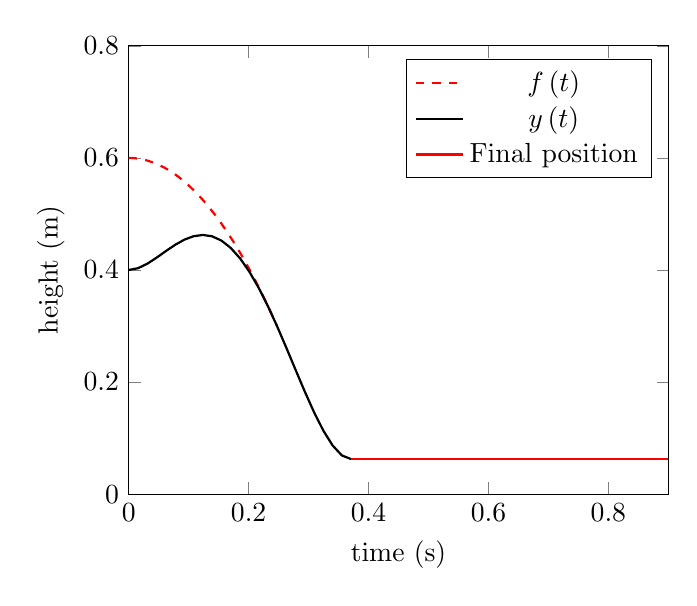
\begin{tikzpicture}
            \begin{axis}[
                    xmin = 0,
                    xmax = 0.9,
                    ymin = 0,
                    ymax = 0.8,
                    xlabel = time (s),
                    ylabel = height (m),
                    legend pos=north east, 
                    ]
                \addplot[domain = 0:0.247298674822, thick, dashed, red]{0.6-0.5*9.81*x^2};
                \addplot[domain = 0:0.37095212, thick]{160.3981*x^4-105.7772*x^3+14.7141*x^2+0.4};
                \addplot[domain = 0.37095212:0.9, red, thick]{0.0625198478831};
                \legend{$f\left(t\right)$, $y\left(t\right)$, Final position};
            \end{axis}
        \end{tikzpicture}   
        \caption{Robot arm height $y$ versus time $t$}\label{fig1}
    \end{figure}
	

	The origin of the height displayed is based on the pivot point of the robot arm. We know the pivot point to be 0.2 meters above the table, and since we never go negative in this graph we know:
	\begin{equation}
	y_{\textrm{min}} > 0.2
	\end{equation}
	So we stop the egg fast enough to clear the table the arm is sitting on, as 0.2 meters is greater than the minimum 0.1 meters given by the problem. This means we stop the catcher at 0.3710 seconds after it starts moving, and 0.1237 seconds after it catches the egg.\newline
    Differentiating $y$, we get the following:
    \begin{equation}\label{y_velocity}
        \dot{y}\left(t\right) = 641.6 \cdot t^3 - 317.34 \cdot t^2 + 29.42 \cdot t
    \end{equation}
    \begin{equation}\label{y_acceleration}
        \ddot{y}\left(t\right) = 1924.8 \cdot t^2 - 634.68 \cdot t + 29.42
    \end{equation}


	Now we just need to convert this $y$ function to polar coordinate to find where our motor should go to. This can be done via the Pythagorean theorem and trigonometry. The value of $r$ tells us the length of the linear actuator in the arm, and the value of $\theta$ tells us the angle of the actuator at the base of the arm (with respect to the horizontal axis). Here, $r$ tells us the length of the linear actuator in the arm, and $\theta$ tells us the angle of the actuator at the base of the arm (with respect to the horizontal axis). 

    \begin{figure}[H]
        \centering
        % stolen from https://tex.stackexchange.com/questions/590760/how-can-i-draw-a-right-triangle-in-latex
        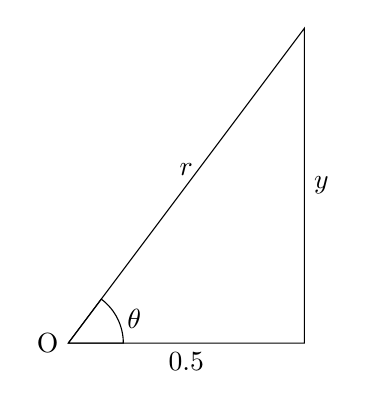
\begin{tikzpicture}
                \coordinate (a) at (7,0);
                \coordinate (b) at (10,0);
                \coordinate (c) at (10,4);
                \draw (a) -- (b)node[midway, below]{0.5} -- (c)node[midway,right]{$y$} -- (a)node[midway,left, above]{$r$ }; % Triangle.
       
                % stolen from https://tex.stackexchange.com/questions/278282/how-to-draw-an-angle-with-tikz#278284
                \draw [] (a) -- ++(0.7cm,0) arc(0:{atan(4/3)}:0.7cm) node[midway,right] {$\theta$} -- cycle;
                \draw (a) node[anchor=east,align=center] {O};
            \end{tikzpicture}
        \caption{Geometric constraints}
    \end{figure}

    These relations give us the following:

    \begin{equation}\label{r_y_1}
        r = \sqrt{0.5^2+y^2} = \sqrt{0.25 + y^2}
	\end{equation}
    \begin{equation}
        \dot{r} = \frac{1}{2\sqrt{0.25+y^2}}\cdot2y\cdot\dot{y} = \frac{ y\cdot\dot{y}}{\sqrt{0.25+y^2}}
	\end{equation}
    \begin{equation}
        \ddot{r} = \frac{y^3 \ddot{y} + 0.25 y\ddot{y} + 0.25\dot{y}^2}{{\left(0.25 + y^2\right)}^{\sfrac{3}{2}}}
	\end{equation}
    For $\theta$, we only care about values between $-\frac{\pi}{2}$ and $\frac{\pi}{2}$.
    \begin{equation}
        \theta = \arctan{\left(\frac{y}{0.5}\right)}
	\end{equation}
    \begin{equation}
        \dot{\theta} = \frac{2\dot{y}}{4y^2 + 1}
	\end{equation}
    \begin{equation}\label{angularAccelEq}
        \ddot{\theta} = \frac{2\ddot{y}\left(4y^2+1\right) - 16y\dot{y}^2}{{\left(4y^2 + 1\right)}^2}
	\end{equation}
    Here, $r$ tells us the length of the linear actuator in the arm, and $\theta$ tells us the angle of the actuator at the base of the arm (with respect to the horizontal axis). We can then add in our function of $y\left(t\right)$ and get the parameters of the actuators as a function of time. 
	\begin{equation}
	r = \sqrt{0.25+\left( 160.4 \cdot t^4 - 105.78 \cdot t^3 + 14.71 \cdot t^2 + 0.4\right)^2}
	\end{equation}
	\begin{equation}
        \theta = \arctan{\left(\frac{160.4 \cdot t^4 - 105.78 \cdot t^3 + 14.71 \cdot t^2 + 0.4}{0.5}\right)}
	\end{equation}
	\begin{equation}
	    \dot{\theta} =\frac{2\cdot\left(641.6\cdot t^3 - 317.34\cdot t^2 + 29.42\cdot t\right)}{4\cdot\left(160.4 \cdot t^4 - 105.78 \cdot t^3 + 14.71 \cdot t^2 + 0.4\right)^2+1}
	\end{equation}

    We can use this information to plot the radius and angle as a function of time. Combining Eq. \eqref{height}, \eqref{y_velocity}, and \eqref{y_acceleration} with Eq. \eqref{r_y_1} to \eqref{angularAccelEq} gives us first and second time derivatives as well, which we can also graph to see how they evolve over time. Note that these graphs cut off when the motion of the robotic arm ends, which would keep the values for the radius and angle constant, while all of their derivatives immediately drop to zero.

    \begin{figure}[H]
        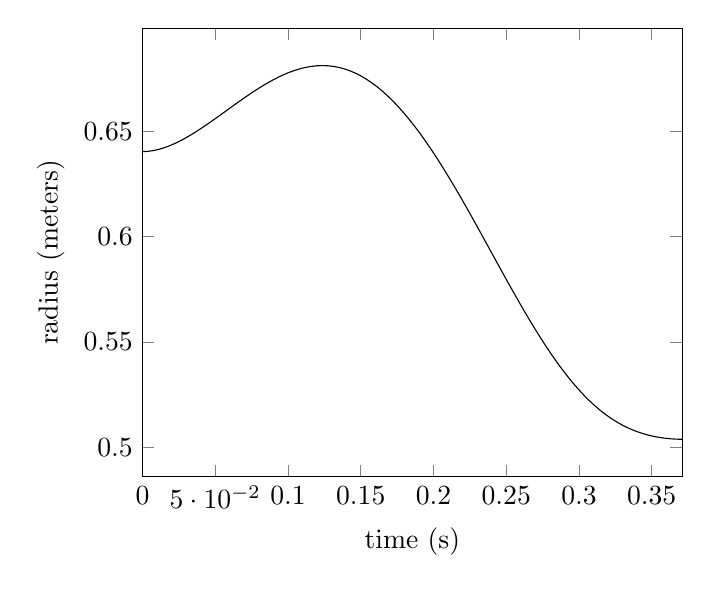
\begin{tikzpicture}
            \begin{axis}[
                    xmin = 0,
                    xmax = 0.37095212,
                    xlabel = time (s),
                    ylabel = radius (meters),
                    legend pos=north east, 
                    samples=100
                    ]
                \addplot[domain = 0:0.37095212]{sqrt(0.25 + f(x)^2)};
            \end{axis}
        \end{tikzpicture}   
        \caption{radius $r$ versus time $t$}\label{figRadius}
    \end{figure}

    \begin{figure}[H]
        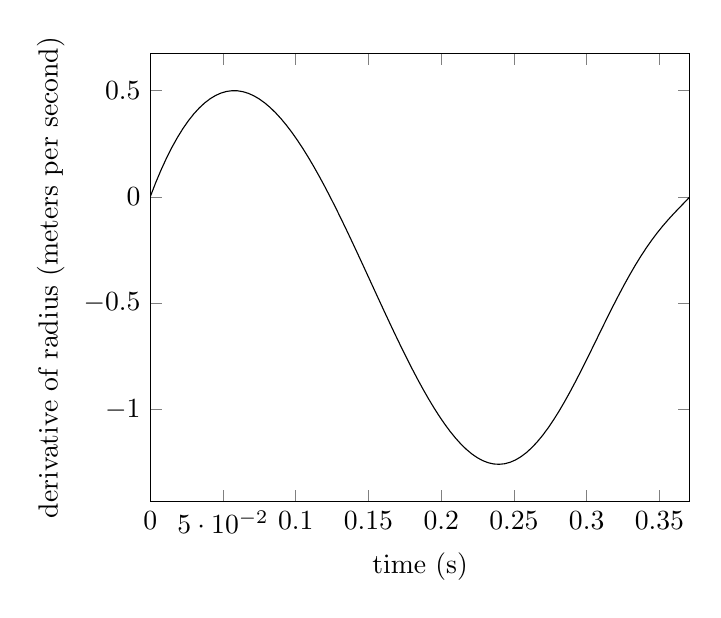
\begin{tikzpicture}
            \begin{axis}[
                    xmin = 0,
                    xmax = 0.37095212,
                    xlabel = time (s),
                    ylabel = derivative of radius (meters per second),
                    legend pos=north east, 
                    samples=100
                    ]
                \addplot[domain = 0:0.37095212]{f(x)*g(x)/sqrt(0.25 + f(x)^2)};
            \end{axis}
        \end{tikzpicture}   
        \caption{first time derivative of radius $\dot{r}$ versus time $t$}
    \end{figure}


    \begin{figure}[H]
        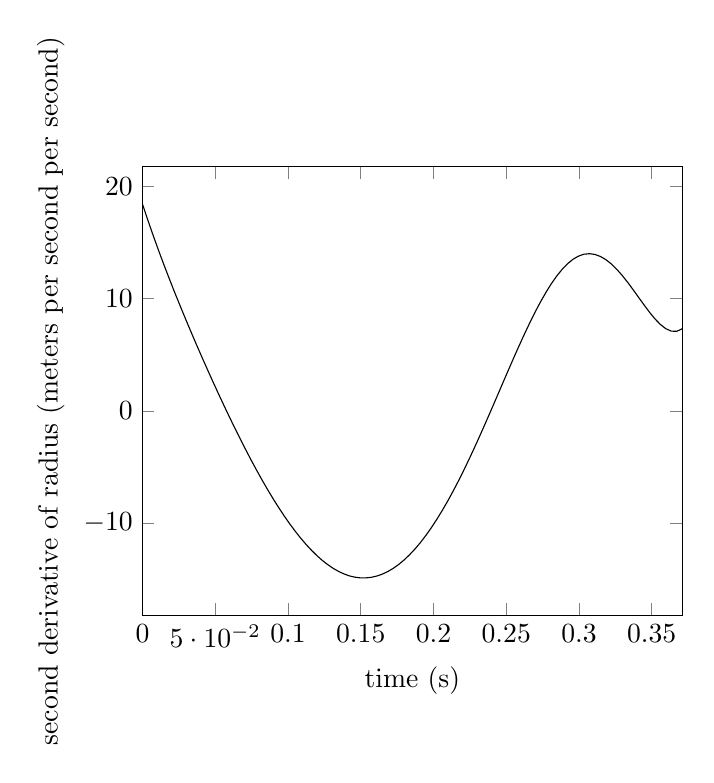
\begin{tikzpicture}
            \begin{axis}[
                    xmin = 0,
                    xmax = 0.37095212,
                    xlabel = time (s),
                    ylabel = second derivative of radius (meters per second per second),
                    legend pos=north east, 
                    samples=100
                    ]
                \addplot[domain = 0:0.37095212]{(f(x)^3*h(x)+0.25*f(x)*h(x)+0.25*(g(x)^2))/((0.25+f(x)^2)^(3/2))};
            \end{axis}
        \end{tikzpicture}   
        \caption{second time derivative of radius $\ddot{r}$ versus time $t$}\label{figRadial_accel}
    \end{figure}


    \begin{figure}[H]
        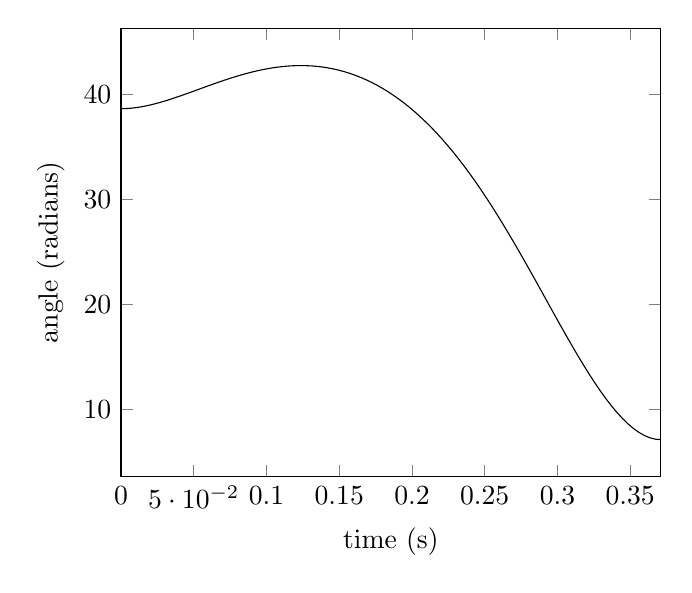
\begin{tikzpicture}
            \begin{axis}[
                    xmin = 0,
                    xmax = 0.37095212,
                    xlabel = time (s),
                    ylabel = angle (radians),
                    legend pos=north east, 
                    samples=100
                    ]
                \addplot[domain = 0:0.37095212]{atan(f(x)/0.5)};
            \end{axis}
        \end{tikzpicture}   
        \caption{angle $\theta$ versus time $t$}
    \end{figure}

    \begin{figure}[H]
        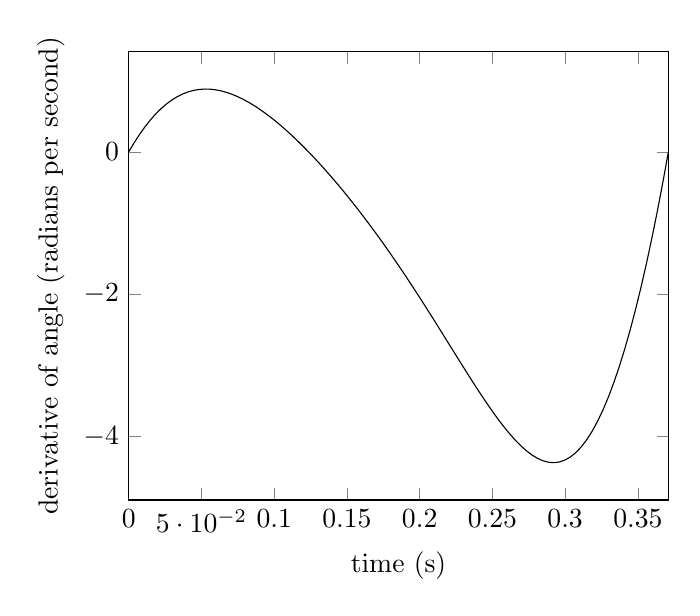
\begin{tikzpicture}
            \begin{axis}[
                    xmin = 0,
                    xmax = 0.37095212,
                    xlabel = time (s),
                    ylabel = derivative of angle (radians per second),
                    legend pos=north east, 
                    samples=100
                    ]
                \addplot[domain = 0:0.37095212]{2*g(x)/(4*f(x)^2+1)};
            \end{axis}
        \end{tikzpicture}   
        \caption{first time derivative of angle $\dot{\theta}$ versus time $t$}
    \end{figure}


    \begin{figure}[H]
        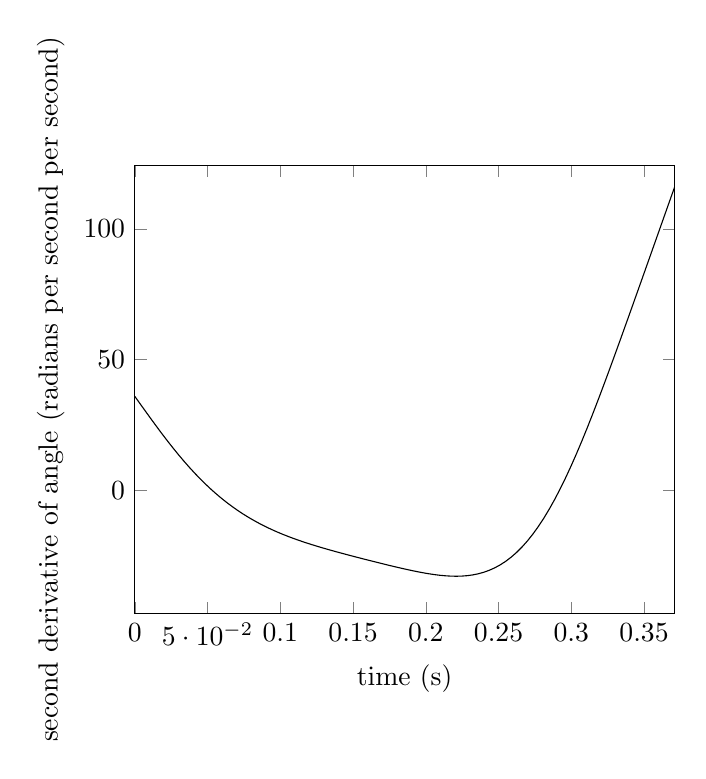
\begin{tikzpicture}
            \begin{axis}[
                    xmin = 0,
                    xmax = 0.37095212,
                    xlabel = time (s),
                    ylabel = second derivative of angle (radians per second per second),
                    legend pos=north east, 
                    samples=100
                    ]
                \addplot[domain = 0:0.37095212]{(2*h(x)*(4*f(x)^2+1)-16*f(x)*g(x)^2)/(4*f(x)^2+1)^2};
            \end{axis}
        \end{tikzpicture}   
        \caption{second time derivative of angle $\ddot{\theta}$ versus time $t$}\label{figAngular_accel}
    \end{figure}


	\section*{Discussion of Results}

        We can combine the components of acceleration shown in Fig. \ref{actuatorAccel3D} and \ref{actuatorAccel2D} with the mass of the egg to determine the forces our solution would impose on an actual actuator. Assuming the mass of the actuator's sliding component and the egg do not exceed 1 kg (likely a conservative estimate), we can get away with an actuator that can exert 20 Newtons of force. The actuator would need to start exerting this force very quickly, though, as radial acceleration starts around 20 meters per second squared. This means the maximum force of the actuator we select would probably need to be higher, and we'd have to look at the force curves to ensure it is capable of this feat. Of course, this actuator would need to have a compressed length about 0.5 meters or less, and a lengthened length of about 0.7 meters or more to fulfill the movement curve, as can be seen in Fig. \ref{figRadius}.

        Something less optimistic towards actually creating this is the tangential acceleration component. Multiplying the second time derivative of the angle with the radius at that moment in time gives us a sideways acceleration. Assuming the linear actuator is rigid, it will need to resist shear and a bending moment, the maximum magnitude of which we can calculate.

        To determine how feasible our rotational profile is, we'd need to know more about how we're rotating our radial actuator. If this is done with another actuator, we'd need to perform calculations to convert these angles into its length. If we used a motor to control it, we'd need to ensure it can output the required torque. Luckily, our initial angular acceleration is about our initial radial acceleration, but isn't at its peak. This means we can likely select a motor/actuator based mostly on its maximum output and just check the torque/force curves to see if it can start at its initial value quickly, as it will have time to ramp up to its maximum value.

        \begin{equation} 
            \vec{\ddot{r}} = \left(\ddot{r} - r{\dot{\theta}}^2\right)\hat{u}_r + \left(r\ddot{\theta} + 2\dot{r}\dot{\theta}\right)\hat{u}_{\theta}
        \end{equation}



        \begin{figure}[H]
            \centering
            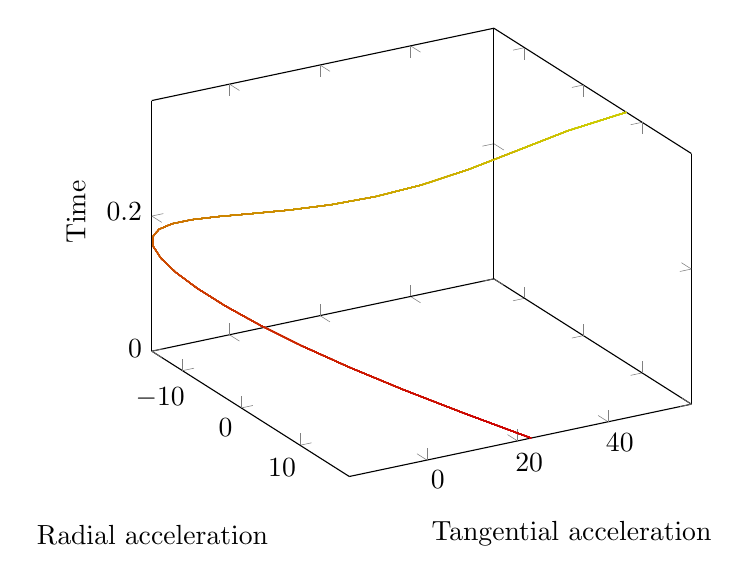
\begin{tikzpicture}
                \begin{axis}[
                        zmin = 0,
                        zmax =  0.37095212,
                        xlabel = Radial acceleration,
                        ylabel = Tangential acceleration,
                        zlabel = Time,
                        view = {60}{30},
                        colormap/autumn,
                        samples = 25 % God help whomever compiles this...
                    ]
                    % radial accel, tangential accel, time, respectively
                    %   parameterized by x (time, in seconds)
                    %   recall, radial accel is \ddot{r} - r(\dot{\theta})^2 
                    %       tangent accel is r \ddot{\theta} + 2 \dot{r} \dot{\theta}
                    % ({x expression},{y expression}, {z expression})
                    \addplot3[domain = 0:0.37095212, no marks, surf]
                        (
                            {(f(x)^3*h(x)+0.25*f(x)*h(x)+0.25*(g(x)^2))/((0.25+f(x)^2)^(3/2)) - sqrt(0.25 + f(x)^2) * (2*g(x)/(4*f(x)^2+1))^2},
                            {sqrt(0.25 + f(x)^2) * (2*h(x)*(4*f(x)^2+1)-16*f(x)*g(x)^2)/(4*f(x)^2+1)^2 + 2 *f(x)*g(x)/sqrt(0.25 + f(x)^2)* 2*g(x)/(4*f(x)^2+1)},
                            {x}
                        );
                \end{axis}
            \end{tikzpicture}

            \caption{Radial and tangential components of acceleration (meters per second squared) over time (seconds)}\label{actuatorAccel3D}
        \end{figure}
        \begin{figure}[H]
            \centering
            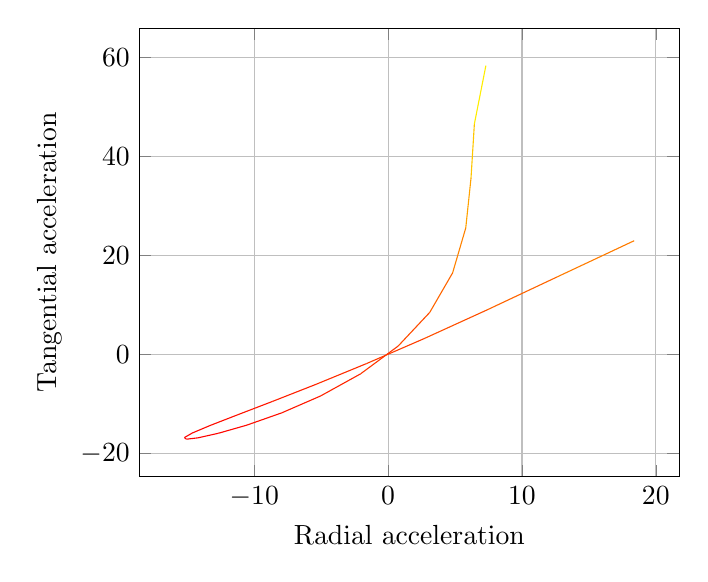
\begin{tikzpicture}
                \begin{axis}[
                        xlabel = Radial acceleration,
                        ylabel = Tangential acceleration,
                        xmajorgrids = true,
                        ymajorgrids = true,
                        colormap/autumn,
                       % samples = 25 % God help whomever compiles this...
                    ]
                    % radial accel, tangential accel, time, respectively
                    %   parameterized by x (time, in seconds)
                    %   recall, radial accel is \ddot{r} - r(\dot{\theta})^2 
                    %       tangent accel is r \ddot{\theta} + 2 \dot{r} \dot{\theta}
                    \addplot[domain = 0:0.37095212, no marks, surf]
                        (
                            {(f(x)^3*h(x)+0.25*f(x)*h(x)+0.25*(g(x)^2))/((0.25+f(x)^2)^(3/2)) - sqrt(0.25 + f(x)^2) * (2*g(x)/(4*f(x)^2+1))^2},
                            {sqrt(0.25 + f(x)^2) * (2*h(x)*(4*f(x)^2+1)-16*f(x)*g(x)^2)/(4*f(x)^2+1)^2 + 2 *(f(x)*g(x)/sqrt(0.25 + f(x)^2))* 2*g(x)/(4*f(x)^2+1)}
                        );
                \end{axis}
            \end{tikzpicture}

            \caption{Radial vs. tangential components of acceleration (meters per second squared))}\label{actuatorAccel2D}
        \end{figure}


        If we were to actually implement this, our solution is set up in such a way that it can be quickly calculated with the given points. Therefore, to allow me to easily update the arm project as I go, I'd likely set these points up as constant values at compile\footnote{For higher level micro-controllers it is possible to use Python, an interpreted language. One could also use MATLAB, another interpreted language. On the one hand, MATLAB lends itself well to matrix calculation. On the other hand, it's MATLAB. Compiled languages like C++ and libraries like \href{https://github.com/g-truc/glm}{glm} allow us to use \texttt{constexpr} to perform linear algebra computations during compile time, which avoids unnecessary computations on the micro-controller at run-time.} time, which allows us to easily adjust and fine-tune our solution path if we need to (if we find we need to catch the egg a little earlier, for example).

	% needs data of actuators
	
\end{document}
